\documentclass[a4paper,12pt]{jarticle}
\usepackage[dvipdfmx]{graphicx}
\usepackage{amsmath}
\usepackage{subfigure}
\usepackage{comment}

\setlength{\hoffset}{0cm}
\setlength{\oddsidemargin}{-3mm}
\setlength{\evensidemargin}{-3cm}
\setlength{\marginparsep}{0cm}
\setlength{\marginparwidth}{0cm}
\setlength{\textheight}{24.7cm}
\setlength{\textwidth}{17cm}
\setlength{\topmargin}{-45pt}

\renewcommand{\baselinestretch}{1.6}
\renewcommand{\floatpagefraction}{1}
\renewcommand{\topfraction}{1}
\renewcommand{\bottomfraction}{1}
\renewcommand{\textfraction}{0}
\renewcommand{\labelenumi}{(\arabic{enumi})}
%\renewcommand{\figurename}{Fig.} %図をFig.にする


%図のキャプションからコロン:を消す
\makeatletter
\long\def\@makecaption#1#2{% #1=図表番号、#2=キャプション本文
\sbox\@tempboxa{#1. #2}
\ifdim \wd\@tempboxa >\hsize
#1 #2\par 
\else
\hb@xt@\hsize{\hfil\box\@tempboxa\hfil}
\fi}
\makeatother
% 


\title{電機システム制御特論 \\
Assignment (2016/05/13)\\
}
\author{\vspace{40mm}\\
九州工業大学大学院 \hspace{0mm} 工学府\\
機械知能工学専攻\ \hspace{0mm} 知能制御工学コース \\
\vspace{5mm}\\
所属:\ 西田研究室\\
学籍番号:\ 16344217\\
提出者氏名:\ 津上 \hspace{0mm} 祐典\\\vspace{5mm}\\ }
\date{平成28年\ 5月\ 20日}

\begin{document}

%表紙
\titlepage
\maketitle
\thispagestyle{empty}

\newpage

%%%%%%%%%%%%%%%%%%%%%%%%
\section{問題}
%%%%%%%%%%%%%%%%%%%%%%%%
DCモータの速度制御系を設計し,4象限運転を実行せよ.ただし,DCモータのパ
ラメータを表\ref{table:DC_dim}に示す.
%
\begin{table}[h]
 \centering
 \caption{DCモータのパラメータ}
 \label{table:DC_dim}
 \begin{tabular}{c|c|c} \hline
  名称 [単位]                    & 記号  & 数値\\\hline
  定格電力 [kW]                  &$P$    &150  \\\hline
  定格電圧 [V]                   &$V$    &450  \\\hline
  電機子抵抗 [$\Omega$]          &$R_a$  & 0.15 \\\hline
  電機子インダクタンス [H]        &$L_a$   &0.003\\\hline
  慣性モーメント [kg$\rm {m^3}$] &$J$     &150  \\\hline
  誘起電圧定数 [V$\cdot$s/rad]    &$K_E$   &8.50 \\\hline
  基底速度 [rpm]                &$\omega$&500  \\\hline
 \end{tabular}
\end{table}
%
%%%%%%%%%%%%%%%%%%%%%%%%
\section{コントローラの設計}
%%%%%%%%%%%%%%%%%%%%%%%%

%%%%%%%%%%%%%%%%%%%%%%%%
\subsection{DCモータ}
%%%%%%%%%%%%%%%%%%%%%%%
はじめに,本レポートで用いるDCモータのブロック線図を図\ref{fig:DC_model}に示す.
%
\begin{figure}[htbp]
 \begin{center}
  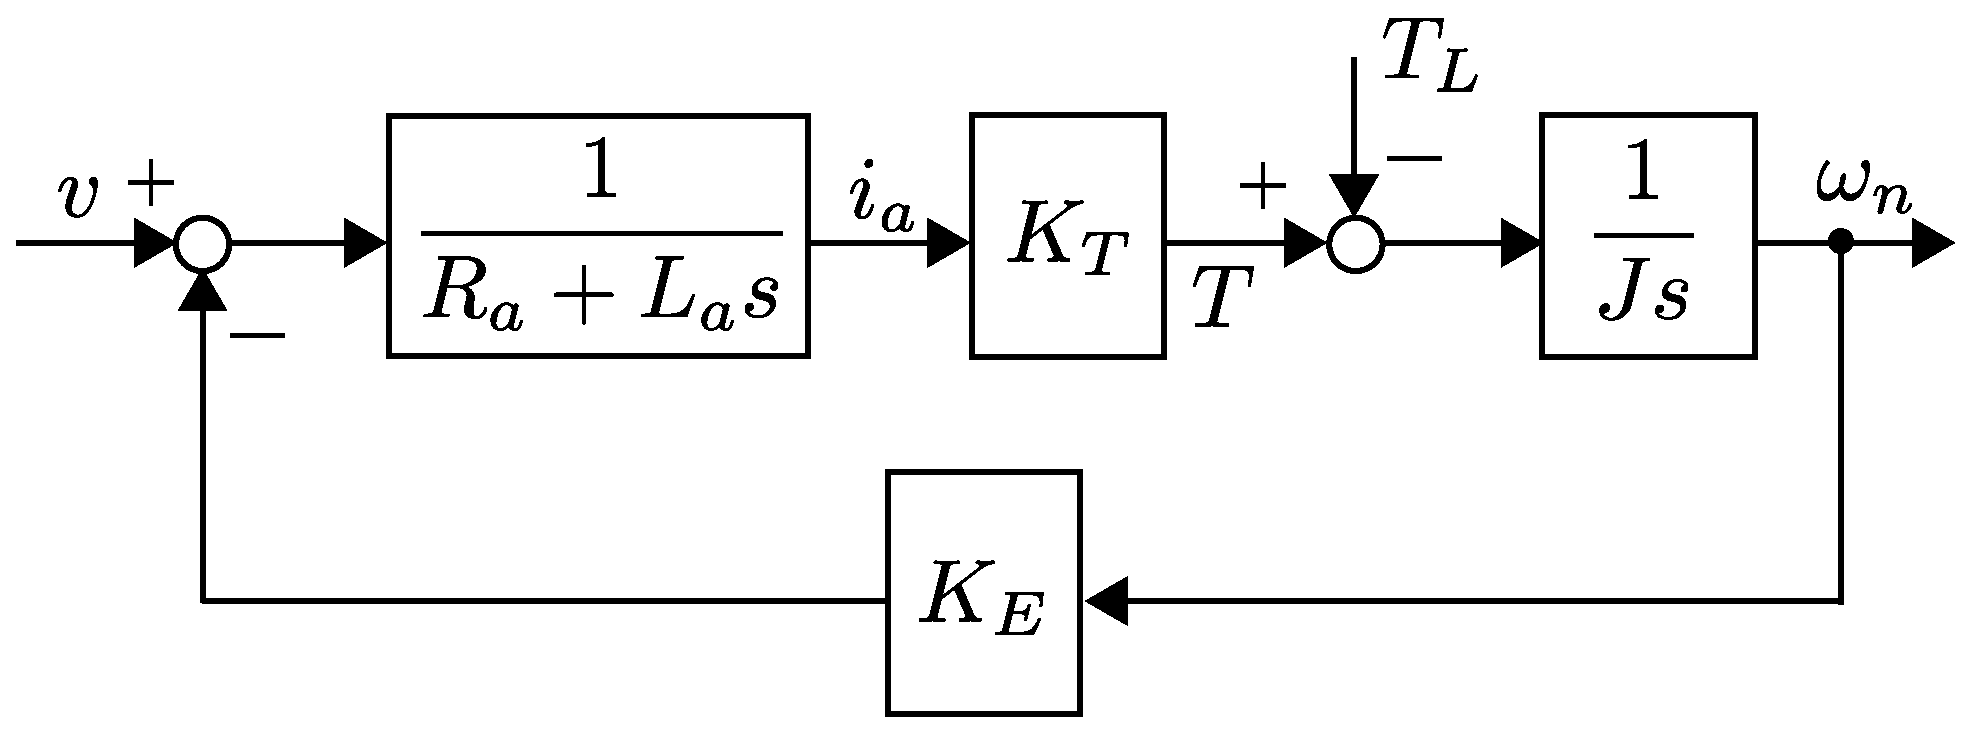
\includegraphics[width = 150mm]{fig/DC_model.eps}
 \end{center}
 \caption{DCモータのブロック線図}
 \label{fig:DC_model}
\end{figure}
%
はじめに,図\ref{fig:DC_model}に示すDCモータのモデルの伝達特性を導出する.
図\ref{fig:DC_model}より
%
\begin{equation}
 \Omega_m(s)=\frac{1}{Js}\left\{\frac{K_T}{R_{a}+L_{a}s}(V-K_E\Omega_m)-T_L\right\}
\end{equation}
と表され,式変形すると,
\begin{equation*}
 \left(Js+\frac{K_{T}K_{E}}{R_{a}+L_{a}}s\right)\Omega_m(s)=\frac{K_{T}}{R_{a}+L_{a}s}-T_L
\end{equation*}
%
\begin{equation*}
 \Omega_m(s)=\frac{K_T}{JL_{a}s^2+JR_{a}s+K_TK_E}-\frac{R_{a}+L_{a}s}{JL_{a}s^2+JR_{a}s+K_TK_E}T_L
\end{equation*}
%
\begin{equation}
 \Omega_m(s)=\frac{\frac{1}{K_E}}{\frac{JL_a}{K_{T}K_E}s^2+\frac{JR_a}{K_{T}K_E}s+1}-\frac{\frac{R_{a}+L_{a}s}{K_{T}K_E}}{\frac{JL_a}{K_{T}K_E}s^2+\frac{JR_a}{K_{T}K_E}s+1}T_L
\end{equation}
%
となる.ここで,(2)式において
\begin{eqnarray}
 \begin{cases}
  T = \sqrt{\frac{L_{a}J}{K_{E}K_T}} & \\
  \zeta= \frac{R_a}{2}\sqrt{\frac{J}{K_{E}K_{T}L_a}} & \\
  K = \frac{1}{K_E}
 \end{cases}
\end{eqnarray}
とおく.すると(2)式は,
\begin{equation}
 \Omega_m(s)=\frac{K}{T^2s^2+2\zeta Ts+1}
\end{equation}
となる.
\end{document}
